\documentclass{standalone}
\usepackage{tikz-network}
\begin{document}
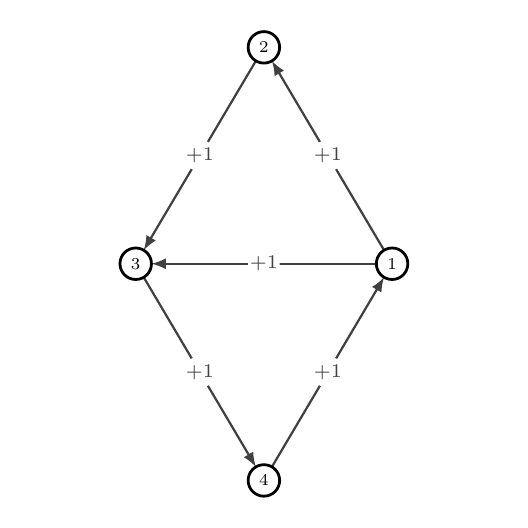
\begin{tikzpicture}
\clip (0,0) rectangle (6,6);
\Vertex[x=4.628,y=3.002,size=0.4,color=white,label=1,fontscale=0.857,shape=circle]{0}
\Vertex[x=3.000,y=5.750,size=0.4,color=white,label=2,fontscale=0.857,shape=circle]{1}
\Vertex[x=1.372,y=3.002,size=0.4,color=white,label=3,fontscale=0.857,shape=circle]{2}
\Vertex[x=3.000,y=0.250,size=0.4,color=white,label=4,fontscale=0.857,shape=circle]{3}
\Edge[,lw=0.8,bend=0,label=+1,Direct](0)(1)
\Edge[,lw=0.8,bend=0,label=+1,Direct](0)(2)
\Edge[,lw=0.8,bend=0,label=+1,Direct](1)(2)
\Edge[,lw=0.8,bend=0,label=+1,Direct](2)(3)
\Edge[,lw=0.8,bend=0,label=+1,Direct](3)(0)
\end{tikzpicture}
\end{document}